\documentclass[11pt,a4paper]{article}

\usepackage{fontspec}
\setmainfont{NotoSansCJKsc-Regular.otf}[
  Path=fonts/,
  BoldFont=NotoSansCJKsc-Bold.otf
]
\setsansfont{NotoSansCJKsc-Regular.otf}[
  Path=fonts/,
  BoldFont=NotoSansCJKsc-Bold.otf
]
\setmonofont{DejaVu Sans Mono}
\XeTeXlinebreaklocale "zh"
\XeTeXlinebreakskip = 0pt plus 1pt

\usepackage[a4paper,top=24mm,bottom=24mm,left=25mm,right=25mm,headheight=15pt]{geometry}
\usepackage{amsmath,amssymb}
\usepackage{graphicx}
\usepackage{booktabs,longtable,tabularx,array,multirow,makecell}
\usepackage{caption,float,placeins}
\usepackage{enumitem}
\usepackage{xcolor}
\usepackage{tcolorbox}
\usepackage{fancyhdr}
\usepackage{titlesec}
\usepackage{hyperref}
\usepackage{setspace}

\definecolor{Primary}{HTML}{1D4ED8}
\definecolor{Secondary}{HTML}{0F766E}
\definecolor{Accent}{HTML}{7C3AED}
\definecolor{Warn}{HTML}{C2410C}
\definecolor{Danger}{HTML}{B91C1C}
\definecolor{Ink}{HTML}{172033}
\definecolor{Muted}{HTML}{64748B}
\definecolor{Panel}{HTML}{F1F5F9}
\definecolor{Rule}{HTML}{CBD5E1}

\hypersetup{
  unicode=true,
  colorlinks=true,
  linkcolor=Primary,
  urlcolor=Secondary,
  citecolor=Accent,
  pdftitle={从FiLM神经动力学场到稀疏岭校准：完整实验演进报告},
  pdfsubject={FBG路面响应反演模型实验报告},
  pdfkeywords={FiLM, 自动微分, 神经场, 路面响应, 稀疏校准, Ridge}
}

\pagestyle{fancy}
\fancyhf{}
\fancyhead[L]{\small FBG 路面响应神经场实验演进}
\fancyhead[R]{\small FiLM $\rightarrow$ Ridge-6 / Gate}
\fancyfoot[C]{\thepage}
\renewcommand{\headrulewidth}{0.4pt}
\renewcommand{\footrulewidth}{0pt}

\titleformat{\section}
  {\Large\bfseries\color{Ink}}{\thesection}{0.65em}{}
  [\vspace{2pt}\color{Rule}\titlerule]
\titleformat{\subsection}
  {\large\bfseries\color{Primary}}{\thesubsection}{0.55em}{}
\titleformat{\subsubsection}
  {\normalsize\bfseries\color{Secondary}}{\thesubsubsection}{0.5em}{}
\titlespacing*{\section}{0pt}{1.4em}{0.8em}
\titlespacing*{\subsection}{0pt}{1.1em}{0.55em}

\setlength{\parindent}{2em}
\setlength{\parskip}{0.25em}
\setlength{\tabcolsep}{5pt}
\renewcommand{\arraystretch}{1.22}
\setlist[itemize]{leftmargin=2em,itemsep=0.25em,topsep=0.35em}
\setlist[enumerate]{leftmargin=2.2em,itemsep=0.3em,topsep=0.35em}
\captionsetup{font=small,labelfont=bf,labelsep=quad}
\renewcommand{\contentsname}{目录}
\renewcommand{\listfigurename}{图目录}
\renewcommand{\listtablename}{表目录}
\renewcommand{\figurename}{图}
\renewcommand{\tablename}{表}
\renewcommand{\abstractname}{摘要}

\newcommand{\ue}{\,\mu\varepsilon}
\newcommand{\rmetrics}[2]{$R^2=#1$，RMSE $=#2\ue$}
\newcommand{\good}[1]{\textcolor{Secondary}{\bfseries #1}}
\newcommand{\bad}[1]{\textcolor{Danger}{\bfseries #1}}
\newcommand{\neutral}[1]{\textcolor{Muted}{#1}}
\newcommand{\method}[1]{\textbf{\textcolor{Primary}{#1}}}
\newcolumntype{Y}{>{\raggedright\arraybackslash}X}
\newcolumntype{C}[1]{>{\centering\arraybackslash}p{#1}}

\newtcolorbox{conclusionbox}{
  colback=blue!4,
  colframe=Primary,
  boxrule=0.8pt,
  arc=2mm,
  left=2mm,right=2mm,top=1.5mm,bottom=1.5mm
}
\newtcolorbox{warningbox}{
  colback=orange!5,
  colframe=Warn,
  boxrule=0.8pt,
  arc=2mm,
  left=2mm,right=2mm,top=1.5mm,bottom=1.5mm
}
\newtcolorbox{methodbox}{
  colback=teal!4,
  colframe=Secondary,
  boxrule=0.8pt,
  arc=2mm,
  left=2mm,right=2mm,top=1.5mm,bottom=1.5mm
}

\begin{document}

\begin{titlepage}
  \centering
  \vspace*{17mm}
  {\color{Primary}\rule{\textwidth}{1.2pt}}\par
  \vspace{13mm}
  {\fontsize{25}{34}\selectfont\bfseries\color{Ink}
  从 FiLM 神经动力学场到稀疏岭校准\par}
  \vspace{5mm}
  {\fontsize{17}{24}\selectfont\color{Primary}
  FBG 路面响应反演模型完整实验演进报告\par}
  \vspace{8mm}
  {\large\color{Muted}
  方法原理、逐步改进、严格对照、95\,cm 极边界分析与最终模型框架\par}
  \vspace{13mm}
  {\color{Primary}\rule{\textwidth}{1.2pt}}\par

  \vfill
  \begin{tcolorbox}[width=0.88\textwidth,colback=Panel,colframe=Rule,boxrule=0.7pt,arc=2mm]
  \centering
  \begin{tabular}{>{\bfseries}p{32mm}p{83mm}}
  基线模型 & Step19 边界感知 FiLM 条件调制 AD-DNF\\
  最终主干 & 原始 Step19-SOTA FiLM 神经动力学场\\
  工况适配 & 6 个稀疏测点的岭仿射校准（Ridge-6）\\
  风险控制 & 6 点留一交叉验证门控，失败时回退 SOTA\\
  数据规模 & 22 个工况，616 条响应记录\\
  报告版本 & 2026 年 7 月实验结果整理版
  \end{tabular}
  \end{tcolorbox}
  \vfill
  {\small\color{Muted}
  本报告中的数值均来自现有 MATLAB 运行输出；早期快速实验与后期严格实验按不同证据等级分别呈现。}
\end{titlepage}

\pagenumbering{roman}
\begin{abstract}
本报告系统整理了 FBG 路面响应反演模型从原始 Step19 FiLM 条件调制神经动力学场，到残差网络、空间边界专家、稀疏岭仿射校准以及稳健门控方案的完整实验演进。原始模型把空间位置与加载工况分别编码，以加载编码产生逐层 FiLM 缩放和平移参数，网络先学习连续位移代理场，再通过自动微分获得与 FBG 对齐的纵、横向应变。该模型在训练集和验证集上分别达到 $R^2=0.9535$ 和 $0.9659$，但独立测试集仅为 $0.7810$；其中 40\,kg 纵中心线 95\,cm 极边界工况为最明显短板，$R^2=0.3703$、RMSE $=202.898\ue$。

为解决该问题，首先进行了 Residual-FiLM 与空间边界专家（MoE 风格）的快速筛选。小规模快速实验曾显示轻微收益，但在恢复 Step19 的网络宽度、FiLM 层数、边界特征、镜像增强、5 折工况级划分和 2400 次迭代后，原始 SOTA 在完整零样本测试上达到 $R^2=0.8467$、RMSE $=79.51\ue$，显著优于 Residual-FiLM 的 $R^2=0.7106$、RMSE $=109.26\ue$。因此，残差与专家结构均未被选作最终主干。

随后将问题从“重建整套网络”转化为“利用少量新工况测点校正系统性幅值与零偏”。在冻结 SOTA 主干后，采用带收缩先验的仿射校准
$\hat y_{\mathrm{cal}}=a\hat y+b$。20 次独立嵌套空间划分的最终实验表明：Ridge-6 的总体 $R^2$ 由 $0.8412$ 提升到 $0.8623$，RMSE 由 $86.63\ue$ 降至 $80.44\ue$，平均下降 $7.15\%$；在 95\,cm 工况上平均降低 $15.78\ue$，20 次中有 85\% 获益。6 点门控方案牺牲部分平均收益，但将总体 RMSE 标准差由 Ridge-6 的 $6.93\ue$ 降至 $2.80\ue$，适合风险更敏感的部署。

\textbf{最终结论：}保留原始 Step19-SOTA FiLM+自动微分神经场作为全局共享主干；若新工况可获得 6 个稀疏测点，则使用 Ridge-6 获得最高平均精度，或使用 Gated Ridge-6 获得更稳健的风险控制。Ridge-4、Residual-FiLM、空间专家和 4 点门控保留为消融实验与方法论证据。
\end{abstract}

\vspace{0.5em}
\noindent\textbf{关键词：} FBG；路面响应反演；FiLM；神经动力学场；自动微分；残差网络；稀疏测点；岭回归；工况适配

\clearpage
\tableofcontents
\clearpage
\listoffigures
\listoftables
\clearpage
\pagenumbering{arabic}

\section{研究问题与实验主线}

\subsection{任务定义}

目标是根据路面空间位置和加载工况，重建连续的结构响应场，并输出可与 FBG 传感器观测直接比较的应变。该任务同时包含两种规律：

\begin{itemize}
  \item \textbf{跨工况共享规律：}不同载荷下路面变形在空间上具有相似的连续结构、对称性和边界效应；
  \item \textbf{工况特异偏差：}某些载荷位置、幅值或极边界条件会使预测整体偏大、偏小或产生零点漂移。
\end{itemize}

原始 FiLM 神经场主要负责第一类规律。后续实验的核心问题是：95\,cm 工况的误差应通过更复杂的共享网络解决，还是通过少量现场测点进行工况级校准解决？

\subsection{总体实验演进}

\begin{figure}[H]
  \centering
  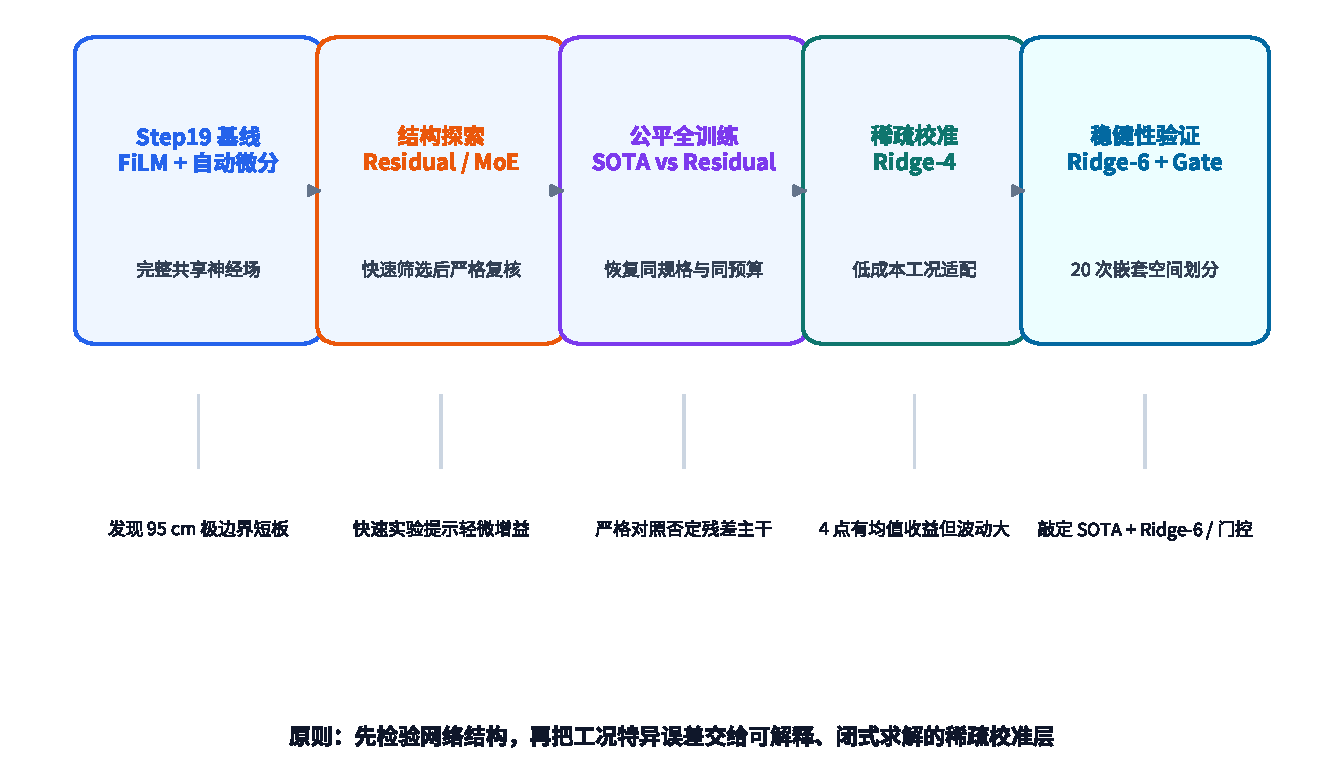
\includegraphics[width=\textwidth]{figures/experiment_evolution.pdf}
  \caption{从原始 FiLM 神经场到最终 Ridge-6 / 门控模型的实验演进}
  \label{fig:evolution}
\end{figure}

整个流程遵循“先结构探索、再公平复核、最后低成本适配”的原则。每一步均设置了明确的保留或淘汰条件，避免仅凭单次结果修改主干。

\begin{table}[H]
\centering
\caption{实验阶段、改进目的与最终决策}
\label{tab:stages}
\small
\begin{tabularx}{\textwidth}{C{13mm} C{25mm} Y Y C{22mm}}
\toprule
阶段 & 方法 & 主要目的 & 证据与意义 & 决策\\
\midrule
Step19 & FiLM + AD-DNF & 建立共享连续响应场 & 训练/验证高，但独立测试和 95\,cm 暴露泛化短板 & 保留为基线\\
结构探索 & Residual-FiLM & 让深层学习增量特征并改善优化 & 快速实验轻微提升；完整训练显著下降 & 淘汰为主干\\
结构探索 & 空间边界专家 & 对边界区域增加专门表达能力 & 相比 Residual 仅微增，参数与训练耗时更高 & 不进入严格全训练\\
稀疏适配 & Ridge-4 & 用 4 点校正比例与零偏 & 单次结果改善，但重复划分波动较大 & 低传感器消融\\
自动选择 & 4 点 LOOCV Gate & 预测校准是否值得应用 & 4 点留一后仅 3 点拟合 2 参数，判别与真实收益负相关 & 淘汰\\
稳健适配 & Ridge-6 & 增加校准约束、降低方差 & 20 次重复平均精度最佳，95\,cm 胜率 85\% & 推荐精度版\\
风险控制 & 6 点 LOOCV Gate & 校准不可靠时回退 SOTA & 仅应用 21.8\%，应用后胜率 79.2\%，总体波动较小 & 推荐稳健版\\
\bottomrule
\end{tabularx}
\end{table}

\section{原始 Step19：边界感知 FiLM 条件调制 AD-DNF}

\subsection{位置编码与加载编码为何要分开}

模型不是简单地把位置与载荷拼成一个向量后直接回归应变，而是将二者赋予不同功能：

\begin{align}
\boldsymbol{s} &= E_s(x,y,d_{\mathrm{edge}},\ldots),\\
\boldsymbol{c} &= E_c(\text{载荷类型},\text{载荷大小},\text{加载位置},\ldots).
\end{align}

其中 $\boldsymbol{s}$ 表示“当前空间点在哪里”，$\boldsymbol{c}$ 表示“当前处于什么加载工况”。空间编码进入共享主干；工况编码不直接替代空间特征，而是生成每一层的调制参数：

\begin{align}
\boldsymbol{\gamma}_\ell,\boldsymbol{\beta}_\ell
  &= G_\ell(\boldsymbol{c}),\\
\boldsymbol{h}_{\ell+1}
  &= \sigma\!\left[
  \boldsymbol{\gamma}_\ell\odot
  (\boldsymbol{W}_\ell\boldsymbol{h}_{\ell}+\boldsymbol{b}_\ell)
  +\boldsymbol{\beta}_\ell
  \right].
\end{align}

这就是 FiLM（Feature-wise Linear Modulation）的作用：同一套空间响应主干被所有工况共享，而不同工况通过 $\gamma$ 和 $\beta$ 对各通道进行缩放与平移。它更接近“在同一物理结构上切换不同加载状态”，而不是为每个工况单独训练一个网络。

\begin{methodbox}
\textbf{对 ResNet 类比的准确表述：}跳连确实让前层表示可直接传到后层，但它不是把“已学特征作为固定先验”冻结下来。后层学习的是相对当前表示的增量；所有层仍通过反向传播共同更新。FiLM 则解决另一维度的问题：它用工况条件改变共享空间主干的行为。
\end{methodbox}

\subsection{位移代理场与自动微分}

模型先输出连续位移代理场
\begin{equation}
w_\theta=w_\theta(x,y;\boldsymbol{c}),
\end{equation}
再在 \texttt{dlfeval} 内保持 $x,y$ 的可追踪计算图，通过二阶自动微分构造应变。薄板/梁式运动学约束可写成
\begin{align}
\varepsilon_x &=-z\frac{\partial^2 w_\theta}{\partial x^2},\\
\varepsilon_y &=-z\frac{\partial^2 w_\theta}{\partial y^2},
\end{align}
其中 $z$ 表示相对于中性面的厚度坐标或等效尺度。该设计的意义是：网络学习一个连续且可微的场，而不是相互独立的离散应变点；纵、横向应变来自同一位移场，因而天然耦合。

\subsection{边界感知设置}

原始报告采用 Asphalt 层、5 个 FiLM 层、空间隐藏维度 96、工况隐藏维度 64，并启用 $x$ 方向镜像增强、边界距离特征与边界加权。极边界阈值为归一化距离 0.210，边界特征长度为 0.180。最优训练轮次为 1071，最优验证数据损失为 0.0553106。

\subsection{原始性能及其正确解释}

\begin{table}[H]
\centering
\caption{原始 Step19 报告中的总体性能}
\label{tab:step19}
\begin{tabular}{lrrrr}
\toprule
数据范围 & $R^2$ & RMSE（$\ue$） & MAE（$\ue$） & Bias（$\ue$）\\
\midrule
训练集 & 0.9535 & 39.400 & 25.278 & -2.155\\
验证集 & 0.9659 & 43.005 & 26.196 & -1.548\\
独立测试集 & 0.7810 & 123.084 & 73.327 & -26.545\\
全部数据 & 0.9164 & 58.712 & 31.955 & -5.398\\
全部数据（排除极边界） & 0.9586 & 40.630 & 25.908 & -2.235\\
\bottomrule
\end{tabular}
\end{table}

\begin{warningbox}
\textbf{为什么“原来 $R^2$ 可达 0.95”而后续只有 0.6--0.8？}
$0.95$ 对应训练集、验证集或排除极边界后的总体统计，并不是严格的未见工况测试指标。原始独立测试集本身只有 $R^2=0.7810$。后续实验采用工况级折分，即测试工况整体不参与训练，难度更高；早期快速包还缩小了网络并显著减少迭代，因此出现 $0.6$--$0.7$ 并不表示原始技术路线失效，而是评估口径和训练预算更严格。
\end{warningbox}

\subsection{95\,cm 极边界短板}

原始报告中最弱工况为 40\,kg 纵中心线 95\,cm 加载：$R^2=0.3703$、RMSE $=202.898\ue$。它的归一化边界距离为 0.208，刚好处于极边界阈值附近。该现象说明：

\begin{enumerate}
  \item 共享主干已学会大多数内部区域和常见工况；
  \item 极边界处响应幅值、曲率或边界约束与训练分布存在差异；
  \item 单纯继续增大共享网络，不一定能以最低代价解决一个局部工况偏差。
\end{enumerate}

\begin{table}[H]
\centering
\caption{原始报告中的部分薄弱工况}
\small
\begin{tabularx}{\textwidth}{Y C{21mm} C{25mm} Y}
\toprule
工况 & $R^2$ & RMSE（$\ue$） & 解释\\
\midrule
40\,kg 纵中心线 95\,cm & 0.3703 & 202.898 & 极边界，首要优化目标\\
5\,kg 单点中心 & 0.5661 & 14.285 & 绝对误差小，但响应方差也小，$R^2$ 敏感\\
10\,kg 单点中心 & 0.7678 & 14.574 & 同属低幅值工况\\
40\,kg 纵中心线 30\,cm & 0.8701 & 52.408 & 边界类工况，但明显优于 95\,cm\\
\bottomrule
\end{tabularx}
\end{table}

\section{第一轮改进：Residual-FiLM 与空间边界专家}

\subsection{Residual-FiLM 的设计意图}

Residual-FiLM 将普通层更新改写为
\begin{equation}
\boldsymbol{h}_{\ell+1}
=\boldsymbol{h}_{\ell}
+F_\ell(\boldsymbol{h}_{\ell};\boldsymbol{c}),
\end{equation}
即保留当前特征并学习增量。预期收益包括更稳定的梯度传播、减少深层退化、让网络专注于“相对已学响应结构的修正”。这对应最初提出的想法：让模型学习整个路面共享结构，并用残差表达工况差异。

但在本任务中，网络最终还要对 $w_\theta$ 做二阶微分。跳连改变的不只是位移拟合，也会改变曲率场的频谱和优化条件；“位移更易拟合”并不自动等价于“二阶导数应变更准确”。

\subsection{空间边界专家 / MoE 思路}

边界专家方案保留共享主干，并增加一个对边界距离敏感的局部专家，再通过门控权重融合：
\begin{equation}
\hat y=(1-g)\hat y_{\mathrm{shared}}+g\hat y_{\mathrm{edge}},
\qquad
g=g(d_{\mathrm{edge}},\boldsymbol{c}).
\end{equation}

其优势是可针对 90\,cm、95\,cm 等区域增加表达能力；风险是专家样本不足、门控错误、额外参数与训练时间增加。由于 95\,cm 只有有限工况，专家网络很容易把“边界规律”和“单个工况噪声”混为一谈。

\subsection{快速筛选实验}

早期 v6 使用 3 折、较小网络（空间宽度 48、条件宽度 32、3 个块）和较短训练，用于快速判断方向，而非最终模型定论。

\begin{table}[H]
\centering
\caption{v6 快速筛选：完整零样本与共同固定测试结果}
\label{tab:quick}
\small
\begin{tabular}{lrrrr}
\toprule
\multirow{2}{*}{方法} &
\multicolumn{2}{c}{完整零样本（616 行）} &
\multicolumn{2}{c}{共同固定测试（484 行）}\\
\cmidrule(lr){2-3}\cmidrule(lr){4-5}
 & $R^2$ & RMSE（$\ue$） & $R^2$ & RMSE（$\ue$）\\
\midrule
Plain-FiLM & 0.6622 & 118.04 & 0.6443 & 127.60\\
Residual-FiLM & 0.6842 & 114.12 & 0.6623 & 124.32\\
空间边界专家 & 0.6864 & 113.71 & 0.6635 & 124.11\\
Residual + Ridge-4 & --- & --- & 0.6970 & 117.76\\
Residual + Ridge-6 & --- & --- & 0.6996 & 117.25\\
\bottomrule
\end{tabular}
\end{table}

快速结果一度提示 Residual 和边界专家可能有效，但空间专家相对 Residual 的 RMSE 仅改善约 $0.4\ue$，训练时间却从 23.06\,s 墠至 39.29\,s，参数由 25,121 增至 30,787。因此，该阶段的正确结论不是“MoE 已优于 SOTA”，而是“残差方向值得做一次与 Step19 完全一致的严格对照，MoE 暂不继续放大”。

\section{第二轮改进：与原始 SOTA 的完全训练对照}

\subsection{为什么必须重做公平实验}

快速包与原始 Step19 在网络宽度、FiLM 层数、折数和迭代次数上不一致。为了回答“结构改动本身是否有效”，v7 恢复了 Step19 兼容设置：空间宽度 96、条件宽度 64、5 个 FiLM 块、边界特征和权重、$x$ 镜像增强、5 折工况级划分、每折 2400 次迭代，并尽可能共享初始化与小批次序列。

\subsection{严格结果：原始 SOTA 明显优于 Residual}

\begin{figure}[H]
  \centering
  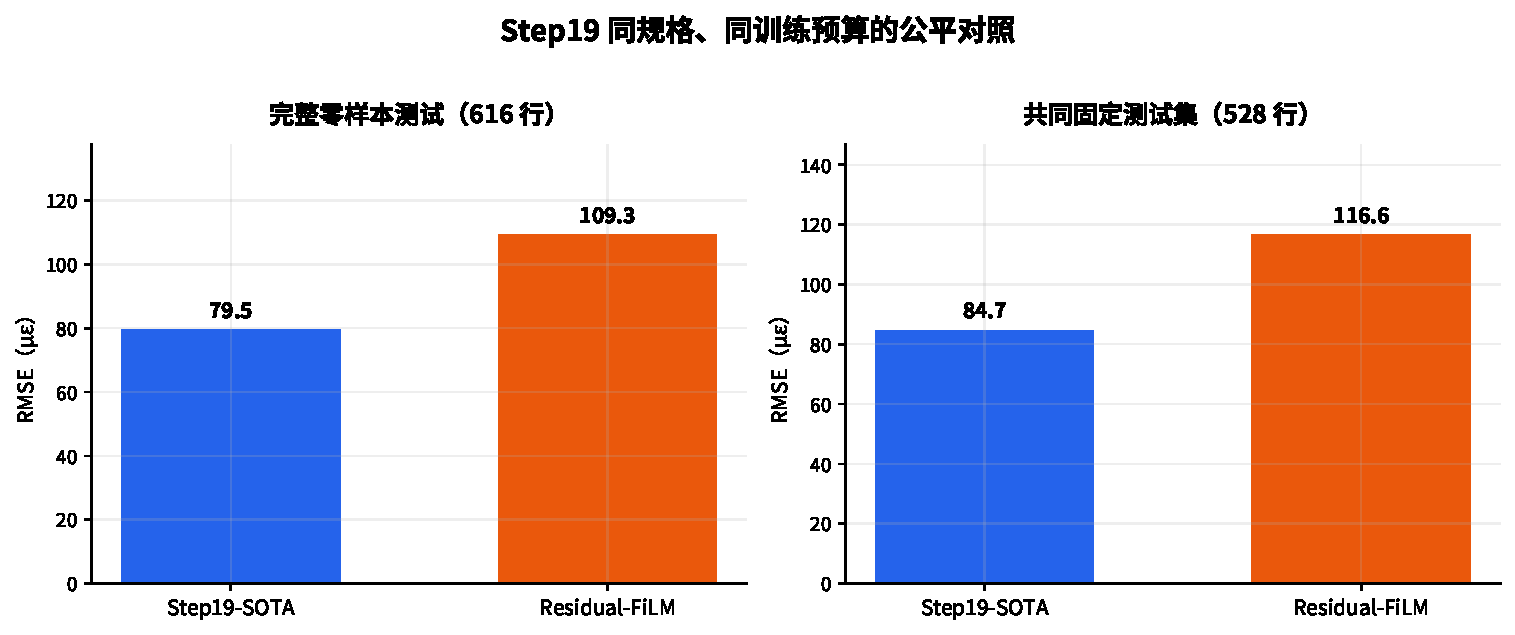
\includegraphics[width=0.92\textwidth]{figures/fair_sota_residual.pdf}
  \caption{Step19 同规格公平对照中，原始 SOTA 的 RMSE 明显低于 Residual-FiLM}
  \label{fig:fair}
\end{figure}

\begin{table}[H]
\centering
\caption{v7 完整训练对照结果}
\label{tab:fair}
\footnotesize
\begin{tabularx}{\textwidth}{C{34mm} Y C{14mm} C{21mm} C{19mm} C{27mm}}
\toprule
测试口径 & 方法 & $R^2$ & RMSE（$\ue$） & MAE（$\ue$） & 最差工况 RMSE（$\ue$）\\
\midrule
\multirow{2}{*}{完整零样本，616 行}
 & Step19-SOTA & \good{0.8467} & \good{79.51} & \good{43.57} & \good{181.74}\\
 & Step19-Residual & 0.7106 & 109.26 & 58.90 & 230.80\\
\midrule
\multirow{3}{*}{共同固定测试，528 行}
 & Step19-SOTA & \good{0.8341} & \good{84.72} & \good{47.20} & \good{195.69}\\
 & Step19-Residual & 0.6859 & 116.56 & 64.24 & 249.13\\
 & Residual + Ridge-4 & 0.7065 & 112.68 & 64.20 & 248.69\\
\bottomrule
\end{tabularx}
\end{table}

完整零样本口径下，Residual 使 RMSE 增加 $29.75\ue$，相对恶化约 37.4\%。共同固定测试上也出现相同趋势。因此，快速实验中的轻微领先属于缩小模型和短训练条件下的局部现象，不能外推到完整 SOTA。

\subsection{收敛与训练时长}

\begin{table}[H]
\centering
\caption{v7 训练时间、推理时间与复杂度}
\label{tab:runtime}
\small
\begin{tabular}{lrrrr}
\toprule
方法 & 平均训练时间（s/折） & 到最佳点时间（s） & 推理（ms/行） & 参数量\\
\midrule
Step19-SOTA & 156.13 & \good{121.14} & 0.267 & 158,529\\
Step19-Residual & \good{148.06} & 129.44 & 0.271 & 158,529\\
Residual + Ridge-4 & 148.06 & 129.44 & 0.271 & 158,531\\
\bottomrule
\end{tabular}
\end{table}

Residual 的总训练时间略短约 5.2\%，但到达其最佳验证点反而更慢，且精度显著更差，因此不能视为有效的效率提升。两者推理耗时基本相同。

逐折最佳验证 RMSE 也一致支持 SOTA：5 折分别为 35.55、67.29、66.56、51.69、59.42；Residual 为 60.86、79.21、70.52、156.35、74.56，尤其第 4 折发生明显退化。

\begin{conclusionbox}
\textbf{阶段决策：}不在整个模型中引入 ResNet，也不把 MoE 作为主干。保留原始 Step19-SOTA，因为它对连续位移场及其二阶导数的联合学习更稳定。后续优化集中在“冻结共享主干后的工况级稀疏校准”。
\end{conclusionbox}

\section{第三轮改进：4--6 个稀疏测点的岭仿射校准}

\subsection{“岭仿射校准”究竟是什么}

对一个新工况，SOTA 主干先给出所有位置的预测 $\hat y_i$。若现场可测得 $k$ 个稀疏点 $(\hat y_i,y_i)$，不重新训练神经网络，只拟合两个参数：
\begin{equation}
\hat y_i^{\,\mathrm{cal}}=a\hat y_i+b.
\end{equation}

$a$ 修正整体幅值比例，$b$ 修正整体零偏。为了避免 4--6 个点把噪声放大，目标函数加入向“无需校准”状态 $(a,b)=(1,0)$ 收缩的岭惩罚：
\begin{equation}
\min_{a,b}
\sum_{i=1}^{k}(y_i-a\hat y_i-b)^2
\lambda_a(a-1)^2+\lambda_b b^2.
\label{eq:ridge}
\end{equation}

现有实验设置为 $\lambda_a=1.0$、$\lambda_b=0.05$，并将比例 $a$ 限制在 $[0.5,1.5]$。该问题只有 2 个未知量，可用闭式线性方程直接求解；校准时间约 $5$--$6\,\mu$s，新增参数仅 2 个。

\begin{methodbox}
\textbf{它不是“用 6 个点重新训练网络”。}神经场的 158,529 个参数全部冻结，6 点只估计比例 $a$ 和偏置 $b$。因此它保留了 SOTA 学到的全路面响应形状，只对新工况的整体幅值和基线做小幅纠正。
\end{methodbox}

\subsection{为什么 6 点通常优于 4 点}

仿射校准有两个自由参数。4 点时每个点都对结果影响很大；若做留一交叉验证，每次仅剩 3 点拟合 2 个参数，门控方差尤其大。6 点使拟合和留一验证分别拥有 6 点和 5 点，虽然仍稀疏，但能够更稳定地区分“系统性偏差”和“单点噪声”。

\subsection{v8：Ridge-4 有收益，4 点门控失败}

\begin{table}[H]
\centering
\caption{v8 单次固定划分结果}
\label{tab:v8}
\small
\begin{tabular}{lrrrrr}
\toprule
方法 & $R^2$ & RMSE（$\ue$） & MAE（$\ue$） & 工况胜数/22 & 平均工况 RMSE 改善\\
\midrule
SOTA & 0.8341 & 84.72 & 47.20 & --- & ---\\
SOTA + Ridge-4 & \good{0.8512} & \good{80.22} & \good{46.10} & 13 & $+3.15\ue$\\
SOTA + Gated Ridge-4 & 0.8337 & 84.80 & 47.83 & 2 & $-0.71\ue$\\
\bottomrule
\end{tabular}
\end{table}

Ridge-4 的单次结果优于基线，但 4 点 LOOCV 门控仅对 4/22 个工况放行，其中 2 个改善、2 个恶化；门控放行时的平均改善反而为 $-3.88\ue$。交叉验证预测收益与实际收益的 Pearson 相关为 $-0.361$、Spearman 相关为 $-0.433$。因此，4 点门控不能可靠预测校准是否有益。

95\,cm 工况在该单次划分中，Ridge-4 把 RMSE 从 $137.21\ue$ 降到 $115.17\ue$，$R^2$ 从 0.7344 提升至 0.8129；但 4 点门控错误拒绝了这次有益校准。这一现象直接推动了 6 点门控与重复划分实验。

\section{第四轮改进：20 次嵌套空间划分的 Ridge-4/6 稳健性实验}

\subsection{实验设计}

v9 不再重新训练神经网络，而是复用 v7 已训练的 5 折 SOTA 模型，专门检验校准点选择的敏感性。对每个工况进行 20 次不重复的嵌套空间划分：

\begin{itemize}
  \item Ridge-4 使用每次排列中的前 4 个测点；
  \item Ridge-6 使用前 6 个测点，因此前 4 点与 Ridge-4 完全相同；
  \item 所有方法在第 6 点之后的同一固定集合上评估；
  \item 共形成 $22\times20=440$ 个“工况--重复”配对。
\end{itemize}

这种嵌套设计排除了“Ridge-6 恰好抽到更容易的测试集”这一混淆因素。

\subsection{总体结果}

\begin{figure}[H]
  \centering
  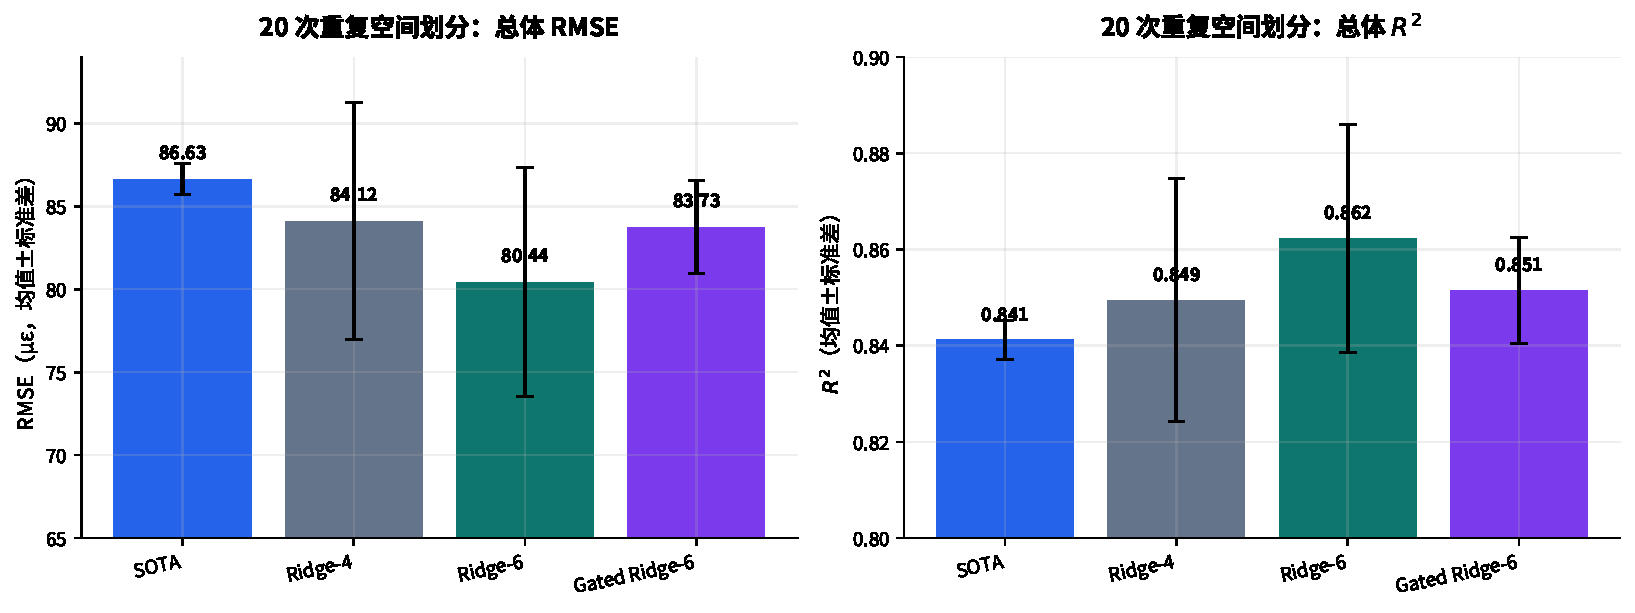
\includegraphics[width=\textwidth]{figures/repeated_global_performance.pdf}
  \caption{20 次重复空间划分下各方法总体性能，误差棒为重复间标准差}
  \label{fig:global-v9}
\end{figure}

\begin{table}[H]
\centering
\caption{v9：20 次重复空间划分的总体结果}
\label{tab:v9global}
\footnotesize
\begin{tabularx}{\textwidth}{Y C{14mm} C{18mm} C{18mm} C{21mm} C{17mm} C{23mm}}
\toprule
方法 & $R^2$ & $R^2$ 标准差 & RMSE（$\ue$） & RMSE 标准差 & MAE（$\ue$） & 相对 RMSE 变化\\
\midrule
SOTA & 0.8412 & 0.0041 & 86.63 & 0.93 & 48.87 & 基线\\
SOTA + Ridge-4 & 0.8495 & 0.0252 & 84.12 & 7.17 & 47.94 & \good{$-2.90\%$}\\
SOTA + Ridge-6 & \good{0.8623} & 0.0237 & \good{80.44} & 6.93 & \good{46.18} & \good{$-7.15\%$}\\
SOTA + Gated Ridge-6 & 0.8515 & 0.0110 & 83.73 & \good{2.80} & 47.30 & \good{$-3.35\%$}\\
\bottomrule
\end{tabularx}
\end{table}

Ridge-6 是平均精度最优方案：相对基线，$R^2$ 平均增加 0.0211，RMSE 降低 $6.19\ue$（7.15\%），MAE 降低 5.51\%。它也明显优于 Ridge-4，证明多出的 2 个校准点提高了约束稳定性。

门控 Ridge-6 的平均收益低于“始终 Ridge-6”，因为它会拒绝一部分实际有益的校准；但其 RMSE 标准差为 $2.80\ue$，远低于始终 Ridge-6 的 $6.93\ue$，体现了风险控制价值。

\subsection{配对胜率与门控审计}

\begin{table}[H]
\centering
\caption{440 个工况--重复配对的改善统计}
\label{tab:paired}
\small
\begin{tabular}{lrrrrr}
\toprule
候选方法 & 平均 RMSE 改善（$\ue$） & 中位改善（$\ue$） & 改善标准差 & 胜数/440 & 胜率\\
\midrule
Ridge-4 & 3.069 & 0.203 & 19.909 & 227 & 51.6\%\\
Ridge-6 & \good{5.483} & \good{1.770} & 18.003 & \good{252} & \good{57.3\%}\\
Gated Ridge-6 & 2.825 & 0 & \good{10.031} & 76 & 17.3\%\\
\bottomrule
\end{tabular}
\end{table}

门控的“总体胜率”不能直接与始终校准比较，因为 344 个被拒绝配对与基线完全相同，改善记为 0。门控实际放行 96/440（21.8\%）；在放行配对中 76 个改善、20 个恶化，条件胜率为 \good{79.2\%}，放行时平均降低 RMSE $12.95\ue$。

\subsection{6 点门控规则}

每个候选工况用 6 点做留一交叉验证，比较校准前后的 CV RMSE。满足以下条件时才应用 Ridge-6，否则回退原始 SOTA：

\begin{enumerate}
  \item 相对 CV 改善至少 5\%；
  \item 绝对 CV 改善至少 $2\ue$；
  \item 拟合比例 $a$ 未逼近限制区间 $[0.5,1.5]$ 的危险边缘。
\end{enumerate}

该门控不是一个新的大模型，而是“使用校准”与“使用原始 SOTA”之间的可审计决策层。

\section{95\,cm 目标工况的最终结果}

\begin{figure}[H]
  \centering
  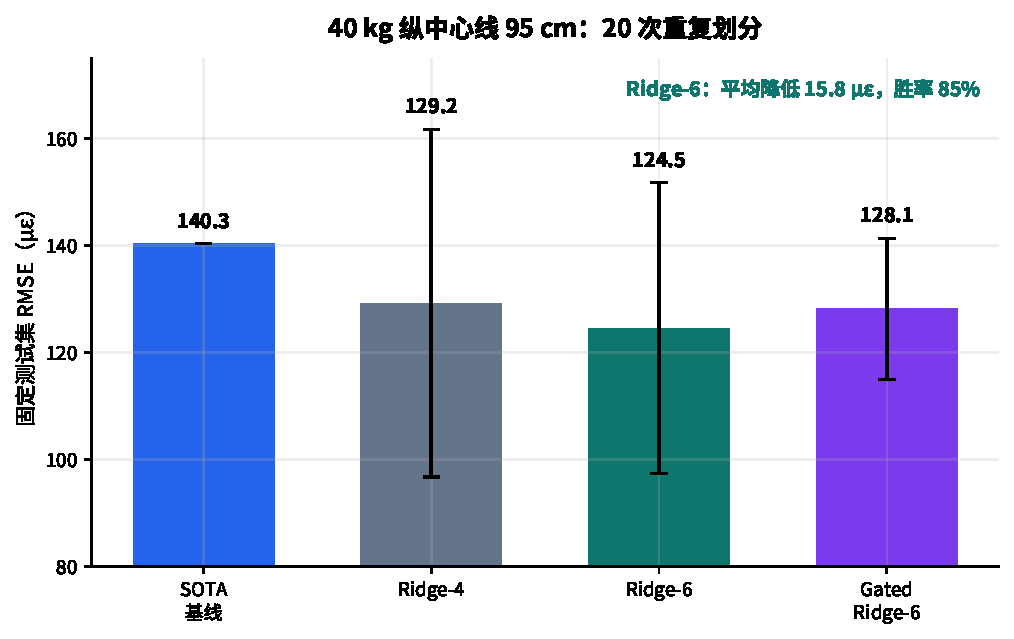
\includegraphics[width=0.78\textwidth]{figures/target_95cm.pdf}
  \caption{95\,cm 工况在 20 次重复空间划分下的固定测试集 RMSE}
  \label{fig:95}
\end{figure}

\begin{table}[H]
\centering
\caption{40\,kg 纵中心线 95\,cm 工况的重复划分结果}
\label{tab:95}
\small
\begin{tabular}{lrrrrrr}
\toprule
方法 & $R^2$ & RMSE（$\ue$） & RMSE 改善 & 胜率 & 改善 P05 & 改善 P95\\
\midrule
SOTA 基线（反推均值） & --- & 140.29 & --- & --- & --- & ---\\
Ridge-4 & 0.7575 & 129.19 & $11.10\ue$ & 85\% & $-47.85\ue$ & $27.61\ue$\\
Ridge-6 & \good{0.7780} & \good{124.50} & \good{$15.78\ue$} & \good{85\%} & $-27.36\ue$ & $30.36\ue$\\
Gated Ridge-6 & 0.7698 & 128.14 & $12.15\ue$ & 50\% & \good{$0.00\ue$} & $28.02\ue$\\
\bottomrule
\end{tabular}
\end{table}

Ridge-6 相对重复实验基线平均降低约 11.25\% 的 RMSE，是 95\,cm 工况的最高平均精度方案。其 P05 仍为负，说明少数校准点组合可能恶化。门控方案平均改善略小，但 P05 为 0：在观察到的 20 次划分中，不可靠校准被回退到基线，因此没有产生负改善。

\begin{conclusionbox}
\textbf{对 95\,cm 问题的回答：}
该工况不需要单独重训一个专家网络。原始 SOTA 已提供可用的空间形状，主要剩余误差可由少量测点纠正幅值和零偏。若追求平均精度，使用 Ridge-6；若极度重视“不能比基线更差”，使用 Gated Ridge-6。
\end{conclusionbox}

\section{分工况规律与适用边界}

\begin{figure}[p]
  \centering
  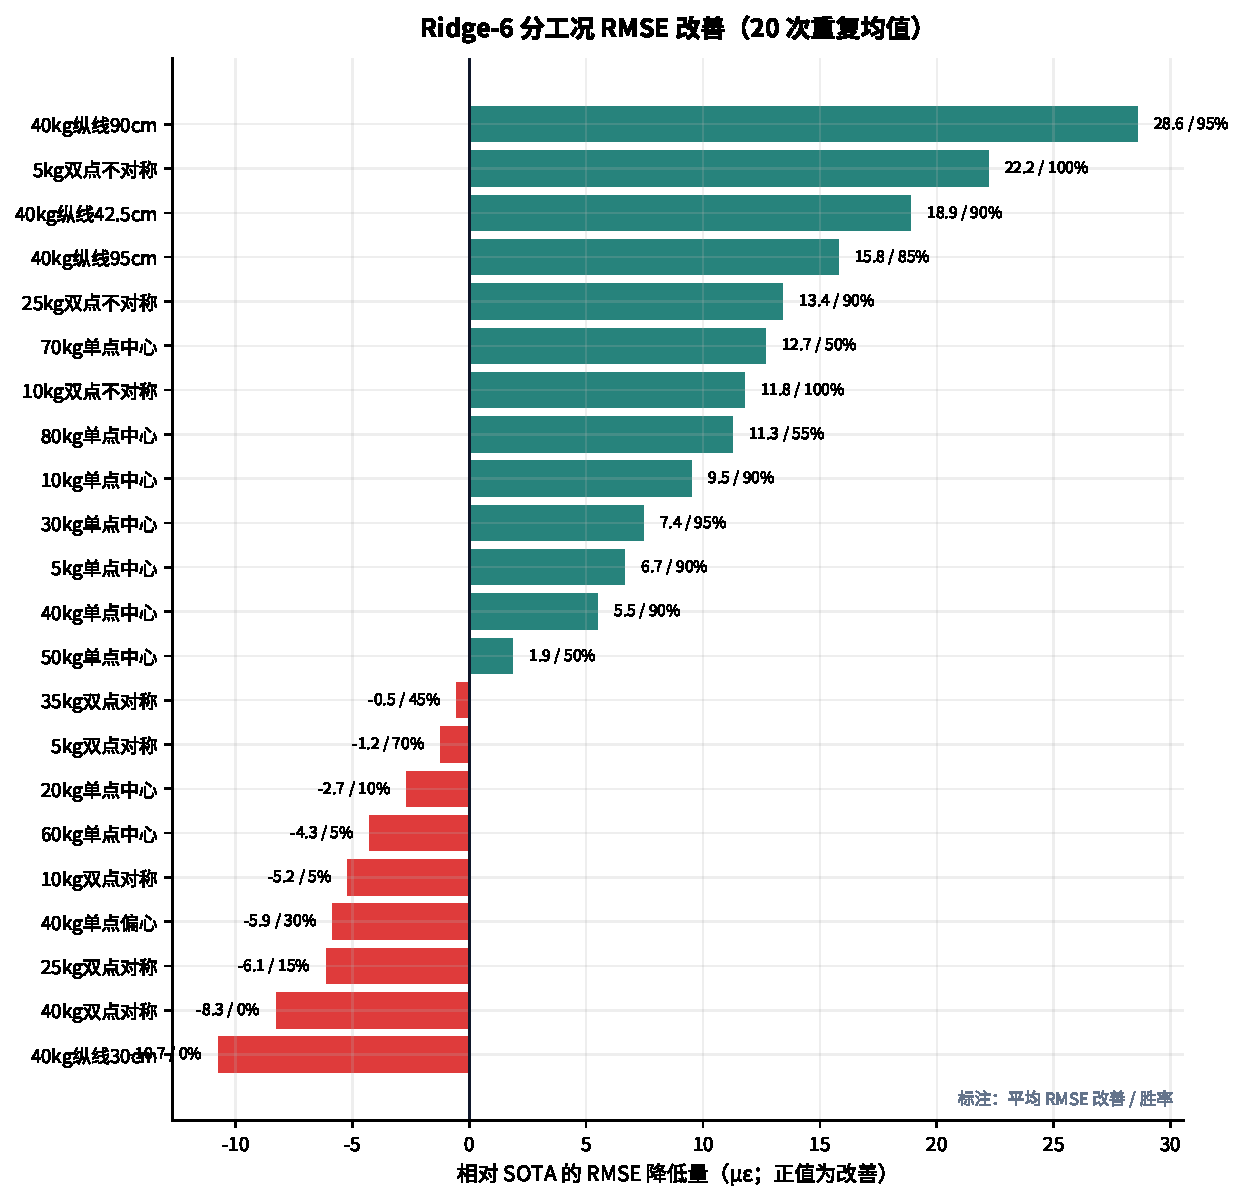
\includegraphics[width=0.88\textwidth]{figures/casewise_ridge6_gain.pdf}
  \caption{Ridge-6 在 22 个工况上的平均 RMSE 改善及胜率}
  \label{fig:casegain}
\end{figure}
\FloatBarrier

\subsection{较稳定受益的工况}

\begin{table}[H]
\centering
\caption{Ridge-6 中平均收益较高或胜率较高的代表工况}
\small
\begin{tabularx}{\textwidth}{Y C{27mm} C{20mm} C{27mm}}
\toprule
工况 & 平均 RMSE 改善（$\ue$） & 胜率 & P05（$\ue$）\\
\midrule
40\,kg 纵中心线 90\,cm & 28.58 & 95\% & -2.04\\
5\,kg 双点不对称 & 22.20 & 100\% & 19.21\\
40\,kg 纵中心线 42.5\,cm & 18.88 & 90\% & -1.92\\
40\,kg 纵中心线 95\,cm & 15.78 & 85\% & -27.36\\
10\,kg 双点不对称 & 11.76 & 100\% & 8.01\\
30\,kg 单点中心 & 7.45 & 95\% & 0.30\\
\bottomrule
\end{tabularx}
\end{table}

不对称加载、90--95\,cm 近边界工况和部分单点中心工况更容易受益，说明它们存在较一致的工况级幅值/零偏误差。

\subsection{可能受损的工况}

\begin{table}[H]
\centering
\caption{Ridge-6 平均收益为负的代表工况}
\small
\begin{tabularx}{\textwidth}{Y C{27mm} C{20mm} Y}
\toprule
工况 & 平均 RMSE 改善（$\ue$） & 胜率 & 解释\\
\midrule
40\,kg 纵中心线 30\,cm & -10.74 & 0\% & 偏差并非简单全局仿射形式\\
40\,kg 双点对称 & -8.26 & 0\% & 原始形状/幅值已较稳定，校准易过修正\\
25\,kg 双点对称 & -6.12 & 15\% & 对校准点位置敏感\\
40\,kg 单点偏心 & -5.86 & 30\% & 可能存在局部形状误差\\
10\,kg 双点对称 & -5.20 & 5\% & 仿射修正收益不足\\
60\,kg 单点中心 & -4.25 & 5\% & 基线已经较强，校准主要引入方差\\
\bottomrule
\end{tabularx}
\end{table}

这些结果表明 Ridge-6 不是对所有工况无条件有效。对于已被主干准确建模的对称工况，少量测点的噪声可能破坏原预测。因此，工程部署可采用以下两种模式：

\begin{itemize}
  \item \textbf{精度优先：}所有有 6 点的工况均使用 Ridge-6，获得总体最高平均精度；
  \item \textbf{风险优先：}使用 6 点门控，仅在校准证据充分时应用，否则维持 SOTA。
\end{itemize}

\section{最终敲定的模型框架}

\subsection{训练阶段}

\begin{enumerate}
  \item 按工况划分训练、验证和测试，避免同一工况的相邻空间点泄漏；
  \item 位置分支编码 $x,y$、边界距离等空间特征；
  \item 加载分支编码载荷类型、大小和位置；
  \item 工况编码产生 5 层 FiLM 的 $\gamma_\ell,\beta_\ell$，调制空间主干；
  \item 网络输出连续位移代理场 $w_\theta$；
  \item 在自动微分图内计算二阶空间导数，得到纵/横向应变；
  \item 使用验证 RMSE 选择检查点，保存全局 SOTA 主干。
\end{enumerate}

\subsection{新工况推理阶段}

\begin{table}[H]
\centering
\caption{最终模型的部署策略}
\begin{tabularx}{\textwidth}{C{31mm} Y Y}
\toprule
可用信息 & 推荐输出 & 适用情形\\
\midrule
无新工况测点 & 原始 Step19-SOTA 零样本预测 & 快速普查、传感器不可用\\
4 个稀疏测点 & Ridge-4（可选） & 传感器极少；作为低成本消融，不建议依赖 4 点门控\\
6 个稀疏测点 & SOTA + Ridge-6 & 平均精度优先\\
6 个稀疏测点且重视风险 & SOTA + Gated Ridge-6 & 校准证据不足时自动回退 SOTA\\
\bottomrule
\end{tabularx}
\end{table}

\subsection{最终选择的意义}

该框架将两类学习任务明确分工：

\begin{itemize}
  \item \textbf{神经场负责形状：}跨工况共享的空间响应结构、连续性、边界信息和运动学耦合；
  \item \textbf{岭校准负责工况偏差：}新工况的整体幅值比例与零偏；
  \item \textbf{门控负责风险：}校准样本不能支持可靠修正时，保持原模型预测。
\end{itemize}

与为 95\,cm 单独训练 MoE 专家相比，该方案参数少、计算快、可解释、可回退，也更适合只有 4--6 个现场测点的小样本现实。

\section{结果汇总与阶段性结论}

\small
\begin{longtable}{@{}C{15mm} C{22mm} C{28mm} p{65mm}@{}}
\caption{完整实验流程的结果与意义汇总}
\label{tab:summary}\\
\toprule
阶段 & 方案 & 关键结果 & 结论及意义\\
\midrule
\endfirsthead
\toprule
阶段 & 方案 & 关键结果 & 结论及意义\\
\midrule
\endhead
原始基线 & Step19 FiLM + AD & 测试 $R^2=0.7810$；95\,cm $R^2=0.3703$ & 主体技术路线有效，但极边界及未见工况泛化仍是瓶颈。\\
\midrule
快速探索 & Plain / Residual / Edge & 零样本 $R^2$：0.662/0.684/0.686 & 小网络短训练下残差略好，只能作为继续实验的信号。\\
\midrule
严格对照 & Step19-SOTA vs Residual & SOTA RMSE 79.51；Residual 109.26 & 恢复完整规格后，原始 SOTA 明显胜出；残差不适合作为最终主干。\\
\midrule
稀疏适配 & Residual + Ridge-4/6 & 快速固定集 RMSE 由 124.32 降至 117.76/117.25 & 仿射适配方向有价值，但应建立在更强的 SOTA 主干上。\\
\midrule
SOTA 校准 & SOTA + Ridge-4 & 单次 RMSE 84.72 $\rightarrow$ 80.22；95\,cm 137.21 $\rightarrow$ 115.17 & 4 点可明显改善部分工况，但稳定性需要重复实验。\\
\midrule
错误门控 & 4 点 LOOCV Gate & 仅 4/22 放行；平均改善 $-0.71\ue$ & 3 点拟合 2 参数的留一验证过于脆弱，门控被否定。\\
\midrule
稳健验证 & 20 次 Ridge-6 & 总体 RMSE 86.63 $\rightarrow$ 80.44；95\,cm 平均降低 15.78 & 6 点为平均精度最优，正式推荐。\\
\midrule
风险控制 & 6 点 Gate & 放行率 21.8\%；放行后胜率 79.2\%；RMSE 标准差 2.80 & 平均收益较小但风险更低，适合保守部署。\\
\bottomrule
\end{longtable}

\section{实验局限与后续工作}

\subsection{当前结论的边界}

\begin{enumerate}
  \item \textbf{数据规模有限：}22 个工况、每工况 28 条记录仍不足以覆盖所有载荷位置和边界条件；
  \item \textbf{重复划分不是新试验：}20 次重复检验的是“测点选择敏感性”，不是 20 次独立物理加载；
  \item \textbf{门控阈值尚需外部验证：}5\% 相对改善、$2\ue$ 绝对改善及比例边界属于当前数据上的工程规则；
  \item \textbf{仿射校准只能修正幅值与零偏：}若误差来自局部峰值位置或形状错位，两个参数无法解决；
  \item \textbf{旧 Step19 与新 5 折结果不应直接横比：}数据划分和评估口径不同，报告中仅用于解释历史现象；
  \item \textbf{分工况规律属于探索性发现：}例如“不对称加载更适合校准”仍需新批次实验确认。
\end{enumerate}

\subsection{建议的下一步}

\begin{enumerate}
  \item 在真实数据上预注册一组完全不参与阈值设计的外部工况，比较 SOTA、Ridge-6 和 Gated Ridge-6；
  \item 对 95\,cm 增加不同载荷大小和重复加载，区分可重复的边界系统偏差与偶然噪声；
  \item 将 6 个测点的空间选择从随机改为覆盖峰值、零交叉和边界的优化设计；
  \item 研究比全局仿射更灵活但仍低维的校准，如分方向双仿射或 2--3 个基函数系数，并严格控制自由度；
  \item 报告置信区间、配对置换检验或 bootstrap 区间，使 Ridge-6 的平均收益具备统计不确定性说明；
  \item 在最终论文中将 Residual、MoE、Ridge-4 和 4 点门控作为消融，说明为何最终选择更简单的 SOTA + Ridge-6。
\end{enumerate}

\section{最终结论}

\begin{conclusionbox}
\begin{enumerate}
  \item 原始“位置编码 + 加载编码 + FiLM 调制 + 位移场 + 自动微分”路线是正确的全局主干；原先的 $R^2\approx0.95$ 主要反映训练/验证或排除极边界后的结果，严格测试水平更接近 $0.78$--$0.85$。
  \item 将 ResNet 加入整个神经动力学场并未改善完整训练结果。Residual-FiLM 在严格零样本测试上从 SOTA 的 $R^2=0.8467$ 降至 0.7106，因此不采用。
  \item 专门边界专家在快速实验中仅比 Residual 略好，成本却显著增加；在样本有限时没有足够证据支持继续扩大 MoE。
  \item 95\,cm 的剩余误差更适合用新工况少量实测点做低维校准。Ridge-6 在 20 次重复中将总体 RMSE 平均降低 7.15\%，并在 95\,cm 工况中平均降低 $15.78\ue$、胜率 85\%。
  \item \textbf{最终框架：}无测点时使用 Step19-SOTA；有 6 点时，精度优先采用 SOTA + Ridge-6，风险优先采用 SOTA + Gated Ridge-6。Ridge-4 保留为测点受限方案，不使用 4 点门控。
\end{enumerate}
\end{conclusionbox}

\appendix
\section{评价指标定义}

\begin{align}
\mathrm{RMSE}
&=\sqrt{\frac{1}{n}\sum_{i=1}^{n}(y_i-\hat y_i)^2},\\
\mathrm{MAE}
&=\frac{1}{n}\sum_{i=1}^{n}|y_i-\hat y_i|,\\
\mathrm{Bias}
&=\frac{1}{n}\sum_{i=1}^{n}(\hat y_i-y_i),\\
R^2
&=1-\frac{\sum_i(y_i-\hat y_i)^2}
{\sum_i(y_i-\bar y)^2}.
\end{align}

对于低幅值工况，$\sum_i(y_i-\bar y)^2$ 很小，因而即使 RMSE 仅十几 $\ue$，$R^2$ 也可能较低甚至为负。报告同时给出 $R^2$ 与 RMSE，避免单一指标误判。

\section{实验版本与文件映射}

\begin{table}[H]
\centering
\caption{代码包版本与用途}
\small
\begin{tabularx}{\textwidth}{C{18mm} C{48mm} Y}
\toprule
版本 & 代码包 & 用途\\
\midrule
初版 & \path{FBG_NeuralField_ResidualMoE_Package} & Plain、Residual、空间边界专家与少样本初测\\
v4 & \path{FBG_NeuralField_FixedFewshot_v4} & 固定测点公平比较\\
v5 & \path{FBG_NeuralField_FinalCalibration_v5} & 校准流程整理\\
v6 & \path{FBG_NeuralField_GlobalBenchmark_v6} & 22 工况快速全局基准、时长与复杂度\\
v7 & \path{FBG_NeuralField_SOTAFullComparison_v7} & Step19 同规格完整训练公平对照\\
v8 & \path{FBG_NeuralField_SOTACalibrationGate_v8} & SOTA + Ridge-4 与 4 点 LOOCV 门控\\
v9 & \path{FBG_NeuralField_SOTARidgeRobustness_v9} & 20 次 Ridge-4/6 嵌套空间稳健性及 6 点门控\\
\bottomrule
\end{tabularx}
\end{table}

\section{报告数据来源}

本报告随附 \texttt{data/} 目录保存了用于正文数值核对的关键 CSV 与原始 Step19 中文分析文本；\texttt{figures/} 目录保存矢量 PDF 和 PNG 图；\texttt{make\_figures.py} 可从这些 CSV 重新生成图表。正文未将早期快速实验结果与后期严格实验结果合并统计。

\vfill
\begin{center}
\color{Muted}\small
—— 报告结束 ——
\end{center}

\end{document}
